% Options for packages loaded elsewhere
\PassOptionsToPackage{unicode}{hyperref}
\PassOptionsToPackage{hyphens}{url}
%
\documentclass[
]{book}
\usepackage{amsmath,amssymb}
\usepackage{lmodern}
\usepackage{iftex}
\ifPDFTeX
  \usepackage[T1]{fontenc}
  \usepackage[utf8]{inputenc}
  \usepackage{textcomp} % provide euro and other symbols
\else % if luatex or xetex
  \usepackage{unicode-math}
  \defaultfontfeatures{Scale=MatchLowercase}
  \defaultfontfeatures[\rmfamily]{Ligatures=TeX,Scale=1}
\fi
% Use upquote if available, for straight quotes in verbatim environments
\IfFileExists{upquote.sty}{\usepackage{upquote}}{}
\IfFileExists{microtype.sty}{% use microtype if available
  \usepackage[]{microtype}
  \UseMicrotypeSet[protrusion]{basicmath} % disable protrusion for tt fonts
}{}
\makeatletter
\@ifundefined{KOMAClassName}{% if non-KOMA class
  \IfFileExists{parskip.sty}{%
    \usepackage{parskip}
  }{% else
    \setlength{\parindent}{0pt}
    \setlength{\parskip}{6pt plus 2pt minus 1pt}}
}{% if KOMA class
  \KOMAoptions{parskip=half}}
\makeatother
\usepackage{xcolor}
\IfFileExists{xurl.sty}{\usepackage{xurl}}{} % add URL line breaks if available
\IfFileExists{bookmark.sty}{\usepackage{bookmark}}{\usepackage{hyperref}}
\hypersetup{
  pdfauthor={Guilherme Baggio},
  hidelinks,
  pdfcreator={LaTeX via pandoc}}
\urlstyle{same} % disable monospaced font for URLs
\usepackage{color}
\usepackage{fancyvrb}
\newcommand{\VerbBar}{|}
\newcommand{\VERB}{\Verb[commandchars=\\\{\}]}
\DefineVerbatimEnvironment{Highlighting}{Verbatim}{commandchars=\\\{\}}
% Add ',fontsize=\small' for more characters per line
\usepackage{framed}
\definecolor{shadecolor}{RGB}{248,248,248}
\newenvironment{Shaded}{\begin{snugshade}}{\end{snugshade}}
\newcommand{\AlertTok}[1]{\textcolor[rgb]{0.94,0.16,0.16}{#1}}
\newcommand{\AnnotationTok}[1]{\textcolor[rgb]{0.56,0.35,0.01}{\textbf{\textit{#1}}}}
\newcommand{\AttributeTok}[1]{\textcolor[rgb]{0.77,0.63,0.00}{#1}}
\newcommand{\BaseNTok}[1]{\textcolor[rgb]{0.00,0.00,0.81}{#1}}
\newcommand{\BuiltInTok}[1]{#1}
\newcommand{\CharTok}[1]{\textcolor[rgb]{0.31,0.60,0.02}{#1}}
\newcommand{\CommentTok}[1]{\textcolor[rgb]{0.56,0.35,0.01}{\textit{#1}}}
\newcommand{\CommentVarTok}[1]{\textcolor[rgb]{0.56,0.35,0.01}{\textbf{\textit{#1}}}}
\newcommand{\ConstantTok}[1]{\textcolor[rgb]{0.00,0.00,0.00}{#1}}
\newcommand{\ControlFlowTok}[1]{\textcolor[rgb]{0.13,0.29,0.53}{\textbf{#1}}}
\newcommand{\DataTypeTok}[1]{\textcolor[rgb]{0.13,0.29,0.53}{#1}}
\newcommand{\DecValTok}[1]{\textcolor[rgb]{0.00,0.00,0.81}{#1}}
\newcommand{\DocumentationTok}[1]{\textcolor[rgb]{0.56,0.35,0.01}{\textbf{\textit{#1}}}}
\newcommand{\ErrorTok}[1]{\textcolor[rgb]{0.64,0.00,0.00}{\textbf{#1}}}
\newcommand{\ExtensionTok}[1]{#1}
\newcommand{\FloatTok}[1]{\textcolor[rgb]{0.00,0.00,0.81}{#1}}
\newcommand{\FunctionTok}[1]{\textcolor[rgb]{0.00,0.00,0.00}{#1}}
\newcommand{\ImportTok}[1]{#1}
\newcommand{\InformationTok}[1]{\textcolor[rgb]{0.56,0.35,0.01}{\textbf{\textit{#1}}}}
\newcommand{\KeywordTok}[1]{\textcolor[rgb]{0.13,0.29,0.53}{\textbf{#1}}}
\newcommand{\NormalTok}[1]{#1}
\newcommand{\OperatorTok}[1]{\textcolor[rgb]{0.81,0.36,0.00}{\textbf{#1}}}
\newcommand{\OtherTok}[1]{\textcolor[rgb]{0.56,0.35,0.01}{#1}}
\newcommand{\PreprocessorTok}[1]{\textcolor[rgb]{0.56,0.35,0.01}{\textit{#1}}}
\newcommand{\RegionMarkerTok}[1]{#1}
\newcommand{\SpecialCharTok}[1]{\textcolor[rgb]{0.00,0.00,0.00}{#1}}
\newcommand{\SpecialStringTok}[1]{\textcolor[rgb]{0.31,0.60,0.02}{#1}}
\newcommand{\StringTok}[1]{\textcolor[rgb]{0.31,0.60,0.02}{#1}}
\newcommand{\VariableTok}[1]{\textcolor[rgb]{0.00,0.00,0.00}{#1}}
\newcommand{\VerbatimStringTok}[1]{\textcolor[rgb]{0.31,0.60,0.02}{#1}}
\newcommand{\WarningTok}[1]{\textcolor[rgb]{0.56,0.35,0.01}{\textbf{\textit{#1}}}}
\usepackage{longtable,booktabs,array}
\usepackage{calc} % for calculating minipage widths
% Correct order of tables after \paragraph or \subparagraph
\usepackage{etoolbox}
\makeatletter
\patchcmd\longtable{\par}{\if@noskipsec\mbox{}\fi\par}{}{}
\makeatother
% Allow footnotes in longtable head/foot
\IfFileExists{footnotehyper.sty}{\usepackage{footnotehyper}}{\usepackage{footnote}}
\makesavenoteenv{longtable}
\usepackage{graphicx}
\makeatletter
\def\maxwidth{\ifdim\Gin@nat@width>\linewidth\linewidth\else\Gin@nat@width\fi}
\def\maxheight{\ifdim\Gin@nat@height>\textheight\textheight\else\Gin@nat@height\fi}
\makeatother
% Scale images if necessary, so that they will not overflow the page
% margins by default, and it is still possible to overwrite the defaults
% using explicit options in \includegraphics[width, height, ...]{}
\setkeys{Gin}{width=\maxwidth,height=\maxheight,keepaspectratio}
% Set default figure placement to htbp
\makeatletter
\def\fps@figure{htbp}
\makeatother
\setlength{\emergencystretch}{3em} % prevent overfull lines
\providecommand{\tightlist}{%
  \setlength{\itemsep}{0pt}\setlength{\parskip}{0pt}}
\setcounter{secnumdepth}{5}
\usepackage{booktabs}
\ifLuaTeX
  \usepackage{selnolig}  % disable illegal ligatures
\fi
\usepackage[]{natbib}
\bibliographystyle{apalike}

\title{\emph{BEYOND ARRAYS}

A brief review of challenges in working with multidimensional downscaled climate data}
\author{Guilherme Baggio}
\date{7 May 2022}

\begin{document}
\maketitle

{
\setcounter{tocdepth}{1}
\tableofcontents
}
\hypertarget{summary}{%
\chapter*{Summary}\label{summary}}
\addcontentsline{toc}{chapter}{Summary}

Much of human society and infrastructure has been built on the assumption that future climate conditions, including average temperature, precipitation, and the frequency and intensity of extreme events, would follow a similar baseline path experienced in the past. Infrastructure design and maintenance, emergency response management, and long-term investment and planning are all affected by this assumption. Human activities, however, are increasing greenhouse gas emissions in the atmosphere. As a result, human-caused climate change is interacting and altering both new and old patterns of climate variability globally. In this context, climate change impact assessments have become a tool to describe these changes and their risks to society. While these assessments frequently deal with the impacts of complex, interconnected systems on local contexts, climate scientists seem to be on the edge of many shifts. For instance, decision-makers are increasingly interested in climate data services that address their local, specific needs. These services are often the result of partnerships between climate scientists and decision-makers, such as city planners, resource managers, health officials, and farmers, involving a range of interactions across multiple fields of study. Climate scientists also have to deal with progressively larger datasets. As high-resolution climate data become available, there has been a proliferation of new approaches to access and manipulate these data. \emph{Pandas}, \emph{xarray}, and \emph{dask}, for instance, are libraries developed to handle complex data structures in the Python ecosystem. Yet, these libraries are considerably recent, and many developers, scientists, and students rely on online forums as a recourse to the frustrating errors caused by the calculations that far exceed the available space in their servers. As a brief contribution to this discussion, this report shares some learnings from working with downscaled climate data. To achieve this goal, \protect\hyperlink{introduction}{Chapter 1} introduces some of the challenges experienced by climate scientists in their attempt to produce fit-for-purpose high-resolution climate data and concisely describes the importance of array programming. \protect\hyperlink{building-a-function-in-xarray}{Chapter 2} provides a step-by-step guide to building a xarray function that enables a parallel execution of calculations. In the context of this study, this function calculates the autocorrelation lag-1 and e-folding time of daily temperature. Finally, the key takeaways summarize some of the development aspects of this study.

\hypertarget{introduction}{%
\chapter{Introduction}\label{introduction}}

\hypertarget{dowscalling-climate-data}{%
\section{Dowscalling climate data}\label{dowscalling-climate-data}}

One of the central issues in the global climate change discussion is the need for regional and local climate data that capture these changes. Such data is required to assess the effects of climate change on human and natural systems, as well as to develop appropriate adaptation and mitigation strategies. Particularly, end-users and decisionmakers have been looking for accurate and reliable climate data to guide response options at the regional and local scales \citep{Overpeck2011, Roberts2018}. This includes high-resolution climate data, reanalysis data, and other monitoring products. For instance, ecosystem and agricultural impact assessments often require high-resolution climate data to assess climate change impacts due to the large spatial variations in natural and agricultural landscapes \citep{NavarroRacines2020, Lafferty2021}, while complex topographies and human-made infrastructures such as mountains, coastlines, lakes, irrigation, and urban heat islands can substantially influence a region's climate and its response to climate forcing \citep{Smid2017, Gutowski2020}.

To bridge this spatial scale gap, various downscaling techniques have been developed to improve low-resolution data from Global Climate Models (GCMs). For instance, \emph{dynamical downscaling} makes use of physically based models, such as GCMs run in limited areas, as boundary conditions to reproduce local climate under different climate change scenarios. These Regional Climate Models (RCMs) are usually computationally intensive, and limited data are available for some regions \citep{DiLuca2015}. Alternatively, \emph{statistical downscaling} relies on a mathematical relationship developed between historic observed climate data and the output of GCMs for the same historical period. This relationship is used to obtain the future downscaled climate data. Statistical downscaling can be also combined with different bias correction methods \citep{Can2015, Wer2016}.

Nonetheless, many challenges have been identified in the long chain that ties climate data from GCMs (and the work of climate scientists) to user-friendly high-resolution climate data that can be used by decisionmakers. The UK Climate Change Act, for example, requires the Environment Agency to report the risks caused by climate change and possible actions to address them. However, identifying and providing climate products for decisionmakers remains a challenge \citep{Orr2021}. By partnering with decisionmakers from different organizations, climate scientists from the Great Lakes Integrated Sciences and Assessments program also observed unrealistic expectations on the development of climate information products \citep{Briley2015}. The challenge of moving from the production of climate information to its use in actual decision-making processes has also been described to as a matter of credibility and legitimacy \citep{Cash2006}, and as a challenge of using uncertain science that has also become highly politicized \citep{Meyer2011}. At the same time, potentially useful climate information often goes unused due to the disparity between what scientists understand as useful information and what end-users recognize as usable in their decision-making processes \citep{Lemos2012}.

\hypertarget{local-data-means-more-data}{%
\section{Local data means more data}\label{local-data-means-more-data}}

Climate scientists face another challenge. As downscaled climate data services become available, such as the \emph{Copernicus Climate Change Service}, operated by the European Centre for Medium-Range Weather Forecasts, and \emph{ClimateData.ca}, a consortium of Canadian governmental and research organizations, the interest towards climate data for specific, local decision-making processes will likely increase \citep{Morand2015, Buontempo2020}. From a computational perspective, this challenge translates to an ``explosion in data from numerical climate model simulations, which have increased greatly in complexity and size'' \citep{Overpeck2011}.

To analyse, process, and present climate data, \emph{array programming} offers a powerful and compact syntax for accessing, manipulating, and operating data. For instance, \_NumPy, the most common array programming library for the Python language, has played a key role in the development of science over the last decades that \citep{Harris2020}. This library developed in the mid-1990s provided a structure that efficiently stores and accesses data in vectors, matrices, and higher-dimensional arrays and enables a wide variety of scientific computations \citep{vanderWalt2011}. It also operates on in-memory arrays using the central processing unit (CPU), which means that the library runs on simple embedded devices as well as the world's largest computers. In this context, the Python ecosystem has proved extremely effective as a platform for climate scientists, and several packages have been developed over time to address specific needs, such as \emph{ClimLab}, \emph{CliMetLab}, \emph{PyGeode}, and \emph{MetPy}.

However, downscaled climate data, as any large dataset, can easily exceed the memory capacity of a single machine. This issue has been accompanied by the emergence of new approaches to handle large amounts of data, including distributed data and parallel execution of graphics processing units (GPUs) and tensor processing units (TPUs). Whereas NumPy's inability to utilize such approaches due to its in-memory data functioning led to a ``gap between available modern hardware architectures and the tools necessary to leverage their computational power'' \citep{Harris2020}, the scientific community's efforts to fill this gap contributed to a proliferation of new array implementations, including \emph{pandas} in 2008, \emph{xarray} in 2014, and \emph{dask} in 2018.

\hypertarget{working-with-xarray}{%
\section{\texorpdfstring{Working with \emph{xarray}}{Working with xarray}}\label{working-with-xarray}}

\hypertarget{building-a-function-in-xarray}{%
\chapter{\texorpdfstring{Building a function in \emph{xarray}}{Building a function in xarray}}\label{building-a-function-in-xarray}}

\hypertarget{working-with-xarray-1}{%
\section{\texorpdfstring{Working with \emph{xarray}}{Working with xarray}}\label{working-with-xarray-1}}

Multi-dimensional arrays are an essential part of computational science. In Python, NumPy provides the fundamental syntax to work with this type of array. However, real-world datasets are usually more than just numbers. They often encode information about the location in space and time across multiple variables and provide qualitative information about of these data. Moreover, large datasets frequently require a faster computational execution of calculations not directly implemented in the NumPy library. In this context, the xarray library provides some of the key functionalities to work with large multi-dimensional arrays.

Firstly, the xarray library introduces the concept of labels in the form of dimensions, coordinates, variables, and attributes assembled on top of NumPy-like arrays. The dimension label specifies the axes of the data, while coordinates are arrays along a dimension. Examples of coordinates include latitude, longitude, days, and months. The variables contain the actual data of the dataset, such as temperature, precipitation, and atmospheric pressure. They are assigned for all the dimensions in a way that associates coordinates with variable values. And the attributes provide the metadata. This structure provides a more intuitive, concise workflow while keeping the well-known NumPy syntax.

Secondly, the xarray library provides tools for working with NetCDF files commonly used in climate sciences. These files allow for storing multi-dimensional data such as temperature and precipitation. Each of these variables can be displayed spatially (by having one value per coordinate of latitude and longitude, for example) and throughout time (by having one value per day, month, or year, for example). The multi-dimensional nature of xarray structures makes them particularly suitable for dealing with labelled scientific data stored in netCDF files. The use of dimension names in xarray instead of NumPy-like axis labels creates a more instinctive coding practice.

To organize the dimensions, coordinates, variables, and attributes of data, the xarray library has two fundamental data structures built upon the strengths of the NumPy and pandas libraries. A \emph{DataArray} is the first structure defined by a multi-dimensional array with an underlying variable. Each DataArray contains dimensions, coordinates, and attributes of one variable only. \emph{Datasets} are the second structure defined by a collection of DataArray objects aligned along with any number of shared dimensions. Since this structure is borrowed from the NetCDF file format, Datasets provide a more natural way to work with data stored in that type of file. Datasets also work as dictionaries, and most operations performed on the dimensions of a DataArray can be performed on Datasets as well.

\hypertarget{creating-a-simple-function-in-xarray}{%
\section{\texorpdfstring{Creating a simple function in \emph{xarray}}{Creating a simple function in xarray}}\label{creating-a-simple-function-in-xarray}}

First, let's import the key libraries for creating a function that calculates the average temperature from daily data for each point in space defined by its coordinates \texttt{latitude} and \texttt{longitude}. This example shows how to use well-known Numpy functions, such as \texttt{mean()} an \texttt{std()}, in a xarray Dataset.

\begin{Shaded}
\begin{Highlighting}[]
\ImportTok{import}\NormalTok{ numpy }\ImportTok{as}\NormalTok{ np}
\ImportTok{import}\NormalTok{ xarray }\ImportTok{as}\NormalTok{ xr}
\end{Highlighting}
\end{Shaded}

The following line uses the command \texttt{xr.open\_dataset} to open the NetCDF file containing daily temperature for one year. This command will be important later when load a large file in chunks. For now, a simple line is sufficient.

\begin{Shaded}
\begin{Highlighting}[]
\NormalTok{t\_daily }\OperatorTok{=}\NormalTok{ xr.open\_dataset(}\StringTok{\textquotesingle{}anusplin\_tasmax\_1year.nc\textquotesingle{}}\NormalTok{)}
\end{Highlighting}
\end{Shaded}

Once we load NetCDF file, we can view all the labels in the Dataset.

\begin{Shaded}
\begin{Highlighting}[]
\NormalTok{t\_daily}
\end{Highlighting}
\end{Shaded}

xarray.Dataset

Dimensions:

{lat}: 510

{lon}: 1068

{time}: 365

Coordinates: {(3)}

{lat}

(lat)

float64

41.04 41.12 41.21 \ldots{} 83.37 83.46

{long\_name :}

lat

{standard\_name :}

latitude

{NAME :}

lat

{units :}

degrees\_north

\_Netcdf4Dimid :

1

{CLASS :}

DIMENSION\_SCALE

{axis :}

Y

{lon}

(lon)

float64

-141.0 -140.9 \ldots{} -52.13 -52.04

{long\_name :}

lon

{standard\_name :}

longitude

{NAME :}

lon

{units :}

degrees\_east

\_Netcdf4Dimid :

0

{CLASS :}

DIMENSION\_SCALE

{axis :}

X

{time}

(time)

datetime64{[}ns{]}

1950-01-01 \ldots{} 1950-12-31

{standard\_name :}

time

{NAME :}

time

\_Netcdf4Dimid :

2

{CLASS :}

DIMENSION\_SCALE

Data variables: {(1)}

{tasmax}

(time, lat, lon)

float32

\ldots{}

{units :}

degC

Attributes: {(14)}

{grid\_resolution :}

Square grid, 0.08333333 degrees\_north by 0.08333333 degrees\_east

\_nc3\_strict :

1

{contact1 :}

Alex Cannon

{contact2 :}

\href{mailto:acannon@uvic.ca}{\nolinkurl{acannon@uvic.ca}}

{title :}

ANUSPLIN interpolated daily minimum temperature, maximum temperature, and precipitation 300 arc second grids

{CDO :}

Climate Data Operators version 1.6.9 (\url{http://mpimet.mpg.de/cdo})

{CDI :}

Climate Data Interface version 1.6.9 (\url{http://mpimet.mpg.de/cdi})

{Conventions :}

CF-1.4

{version\_comment :}

141.00 to 52.00 W, 41.00 to 84.00 N

{version :}

ANUSPLIN data obtained 2 April 2012, 14 June 2012, and 30 January 2013 from Pia Papadopol (\href{mailto:pia.papadopol@nrcan-rncan.gc.ca}{\nolinkurl{pia.papadopol@nrcan-rncan.gc.ca}})

{NCO :}

netCDF Operators version 4.7.5 (Homepage = \url{http://nco.sf.net}, Code = \url{http://github.com/nco/nco})

{input\_data :}

{[}pcp,min,max{]}YYY\_DOY.asc ASCII grid files

{reference :}

McKenney, D.W., et al., 2011. Customized Spatial Climate Models for North America. Bulletin of the American Meteorological Society, 92(12):1611-1622.

{history :}

Thu Jan 27 15:50:07 2022: ncks -d time,0,364 anusplin\_tasmax\_final.nc test.nc
Fri Aug 05 10:39:54 2016: cdo -b f32 copy anusplin\_tasmax.nc anusplin\_tasmax\_unpack.nc
Fri Aug 5 10:03:40 2016: ncks -v tasmax anusplin\_300\_canada\_daily\_standard\_grids\_1950-2010.nc anusplin\_tasmax.nc

The xarray library allows for using most of the functions available in the pandas library, such as the command \texttt{groupby()}, with the advantage of relying on the dimension labels to execute the NumPy function. For example, it is possible to easily calculate the weekly average temperature.

\begin{Shaded}
\begin{Highlighting}[]
\NormalTok{t\_week }\OperatorTok{=}\NormalTok{ t\_daily.groupby(}\StringTok{\textquotesingle{}time.week\textquotesingle{}}\NormalTok{).mean(}\StringTok{\textquotesingle{}time\textquotesingle{}}\NormalTok{).rename(\{}\StringTok{"tasmax"}\NormalTok{: }\StringTok{"t\_mean"}\NormalTok{\})}
\end{Highlighting}
\end{Shaded}

xarray.Dataset

Dimensions:

{lat}: 510

{lon}: 1068

{week}: 52

Coordinates: {(3)}

{lat}

(lat)

float64

41.04 41.12 41.21 \ldots{} 83.37 83.46

{long\_name :}

lat

{standard\_name :}

latitude

{NAME :}

lat

{units :}

degrees\_north

\_Netcdf4Dimid :

1

{CLASS :}

DIMENSION\_SCALE

{axis :}

Y

{lon}

(lon)

float64

-141.0 -140.9 \ldots{} -52.13 -52.04

{long\_name :}

lon

{standard\_name :}

longitude

{NAME :}

lon

{units :}

degrees\_east

\_Netcdf4Dimid :

0

{CLASS :}

DIMENSION\_SCALE

{axis :}

X

{week}

(week)

int64

1 2 3 4 5 6 7 \ldots{} 47 48 49 50 51 52

Data variables: {(1)}

{t\_mean}

(week, lat, lon)

float32

nan nan nan nan \ldots{} nan nan nan nan

Attributes: {(0)}

As we can see, this code automatically adds a new dimension \texttt{week} to the Dataset. Similarly, we can calculate the monthly average temperature.

\begin{Shaded}
\begin{Highlighting}[]
\NormalTok{t\_month }\OperatorTok{=}\NormalTok{ t\_daily.groupby(}\StringTok{\textquotesingle{}time.month\textquotesingle{}}\NormalTok{).mean(}\StringTok{\textquotesingle{}time\textquotesingle{}}\NormalTok{).rename(\{}\StringTok{"tasmax"}\NormalTok{: }\StringTok{"t\_mean"}\NormalTok{\})}
\end{Highlighting}
\end{Shaded}

xarray.Dataset

Dimensions:

{lat}: 510

{lon}: 1068

{month}: 12

Coordinates: {(3)}

{lat}

(lat)

float64

41.04 41.12 41.21 \ldots{} 83.37 83.46

{long\_name :}

lat

{standard\_name :}

latitude

{NAME :}

lat

{units :}

degrees\_north

\_Netcdf4Dimid :

1

{CLASS :}

DIMENSION\_SCALE

{axis :}

Y

{lon}

(lon)

float64

-141.0 -140.9 \ldots{} -52.13 -52.04

{long\_name :}

lon

{standard\_name :}

longitude

{NAME :}

lon

{units :}

degrees\_east

\_Netcdf4Dimid :

0

{CLASS :}

DIMENSION\_SCALE

{axis :}

X

{month}

(month)

int64

1 2 3 4 5 6 7 8 9 10 11 12

Data variables: {(1)}

{t\_mean}

(month, lat, lon)

float32

nan nan nan nan \ldots{} nan nan nan nan

Attributes: {(0)}

As seen in the codes above, the command \texttt{mean(\textquotesingle{}time\textquotesingle{})} is executing the NumPy function \texttt{mean} on the the time dimension of the Dataset and automatically creating a new dimension \texttt{month} with 12 elements. We can now plot the monthly mean temperature.

\begin{Shaded}
\begin{Highlighting}[]
\NormalTok{fig, axs }\OperatorTok{=}\NormalTok{ plt.subplots(}\DecValTok{4}\NormalTok{,}\DecValTok{3}\NormalTok{, figsize}\OperatorTok{=}\NormalTok{(}\DecValTok{12}\NormalTok{, }\DecValTok{16}\NormalTok{), facecolor}\OperatorTok{=}\StringTok{\textquotesingle{}w\textquotesingle{}}\NormalTok{, edgecolor}\OperatorTok{=}\StringTok{\textquotesingle{}k\textquotesingle{}}\NormalTok{)}
\NormalTok{fig.subplots\_adjust(hspace }\OperatorTok{=} \FloatTok{.0}\NormalTok{, wspace}\OperatorTok{=} \FloatTok{.2}\NormalTok{)}

\NormalTok{month }\OperatorTok{=}\NormalTok{ [}\StringTok{\textquotesingle{}JAN\textquotesingle{}}\NormalTok{,}\StringTok{\textquotesingle{}FEB\textquotesingle{}}\NormalTok{,}\StringTok{\textquotesingle{}MAR\textquotesingle{}}\NormalTok{,}\StringTok{\textquotesingle{}APR\textquotesingle{}}\NormalTok{,}\StringTok{\textquotesingle{}MAY\textquotesingle{}}\NormalTok{,}\StringTok{\textquotesingle{}JUN\textquotesingle{}}\NormalTok{,}\StringTok{\textquotesingle{}JUL\textquotesingle{}}\NormalTok{,}\StringTok{\textquotesingle{}AUG\textquotesingle{}}\NormalTok{,}\StringTok{\textquotesingle{}SEP\textquotesingle{}}\NormalTok{,}\StringTok{\textquotesingle{}OCT\textquotesingle{}}\NormalTok{,}\StringTok{\textquotesingle{}NOV\textquotesingle{}}\NormalTok{,}\StringTok{\textquotesingle{}DEC\textquotesingle{}}\NormalTok{]}

\NormalTok{axs }\OperatorTok{=}\NormalTok{ axs.ravel()}

\ControlFlowTok{for}\NormalTok{ i }\KeywordTok{in} \BuiltInTok{range}\NormalTok{(}\BuiltInTok{len}\NormalTok{(month)):}
\NormalTok{    pc }\OperatorTok{=}\NormalTok{ axs[i].pcolormesh(t\_month.lon,t\_month.lat,t\_month[}\StringTok{\textquotesingle{}t\_mean\textquotesingle{}}\NormalTok{][i,:,:],cmap}\OperatorTok{=}\StringTok{"Reds"}\NormalTok{,vmin}\OperatorTok{={-}}\DecValTok{40}\NormalTok{,vmax}\OperatorTok{=}\DecValTok{30}\NormalTok{)}
\NormalTok{    axs[i].set\_title(month[i])}
\NormalTok{    axs[i].set\_ylim([}\DecValTok{39}\NormalTok{,}\DecValTok{81}\NormalTok{])}
\NormalTok{    axs[i].set\_xlim([}\OperatorTok{{-}}\DecValTok{141}\NormalTok{,}\OperatorTok{{-}}\DecValTok{59}\NormalTok{])}

    \ControlFlowTok{if}\NormalTok{ i }\KeywordTok{in}\NormalTok{ [}\DecValTok{0}\NormalTok{,}\DecValTok{3}\NormalTok{,}\DecValTok{6}\NormalTok{,}\DecValTok{9}\NormalTok{]:}
\NormalTok{        axs[i].set\_yticks([}\DecValTok{40}\NormalTok{,}\DecValTok{50}\NormalTok{,}\DecValTok{60}\NormalTok{,}\DecValTok{70}\NormalTok{,}\DecValTok{80}\NormalTok{])}
    \ControlFlowTok{else}\NormalTok{:}
\NormalTok{        axs[i].set\_yticks([])}

    \ControlFlowTok{if}\NormalTok{ i }\KeywordTok{in}\NormalTok{ [}\DecValTok{9}\NormalTok{,}\DecValTok{10}\NormalTok{,}\DecValTok{11}\NormalTok{]:}
\NormalTok{        axs[i].set\_xticks([}\OperatorTok{{-}}\DecValTok{140}\NormalTok{,}\OperatorTok{{-}}\DecValTok{120}\NormalTok{,}\OperatorTok{{-}}\DecValTok{100}\NormalTok{,}\OperatorTok{{-}}\DecValTok{80}\NormalTok{,}\OperatorTok{{-}}\DecValTok{60}\NormalTok{])}
    \ControlFlowTok{else}\NormalTok{:}
\NormalTok{        axs[i].set\_xticks([])                }
        
\NormalTok{fig.suptitle(}\StringTok{\textquotesingle{}Monthly Mean Temperature ($\^{}\{\textbackslash{}circ\}$C)\textquotesingle{}}\NormalTok{,}
\NormalTok{             x}\OperatorTok{=}\FloatTok{0.5}\NormalTok{,y}\OperatorTok{=}\FloatTok{1.0}\NormalTok{,fontsize}\OperatorTok{=}\DecValTok{18}\NormalTok{,fontweight}\OperatorTok{=}\StringTok{"bold"}\NormalTok{)}

\NormalTok{cax,kw }\OperatorTok{=}\NormalTok{ mpl.colorbar.make\_axes(axs,location}\OperatorTok{=}\StringTok{\textquotesingle{}bottom\textquotesingle{}}\NormalTok{,pad}\OperatorTok{={-}}\FloatTok{0.48}\NormalTok{,shrink}\OperatorTok{=}\FloatTok{0.4}\NormalTok{)}
\NormalTok{out}\OperatorTok{=}\NormalTok{fig.colorbar(pc,cax}\OperatorTok{=}\NormalTok{cax,extend}\OperatorTok{=}\StringTok{\textquotesingle{}both\textquotesingle{}}\NormalTok{,}\OperatorTok{**}\NormalTok{kw)}

\NormalTok{out.set\_label(}\StringTok{"Temperature ($\^{}\{\textbackslash{}circ\}$C)"}\NormalTok{, fontweight}\OperatorTok{=}\StringTok{\textquotesingle{}bold\textquotesingle{}}\NormalTok{,fontsize}\OperatorTok{=}\DecValTok{14}\NormalTok{)}

\NormalTok{fig.tight\_layout()}
\NormalTok{plt.show()}
\end{Highlighting}
\end{Shaded}

\begin{figure}
\centering
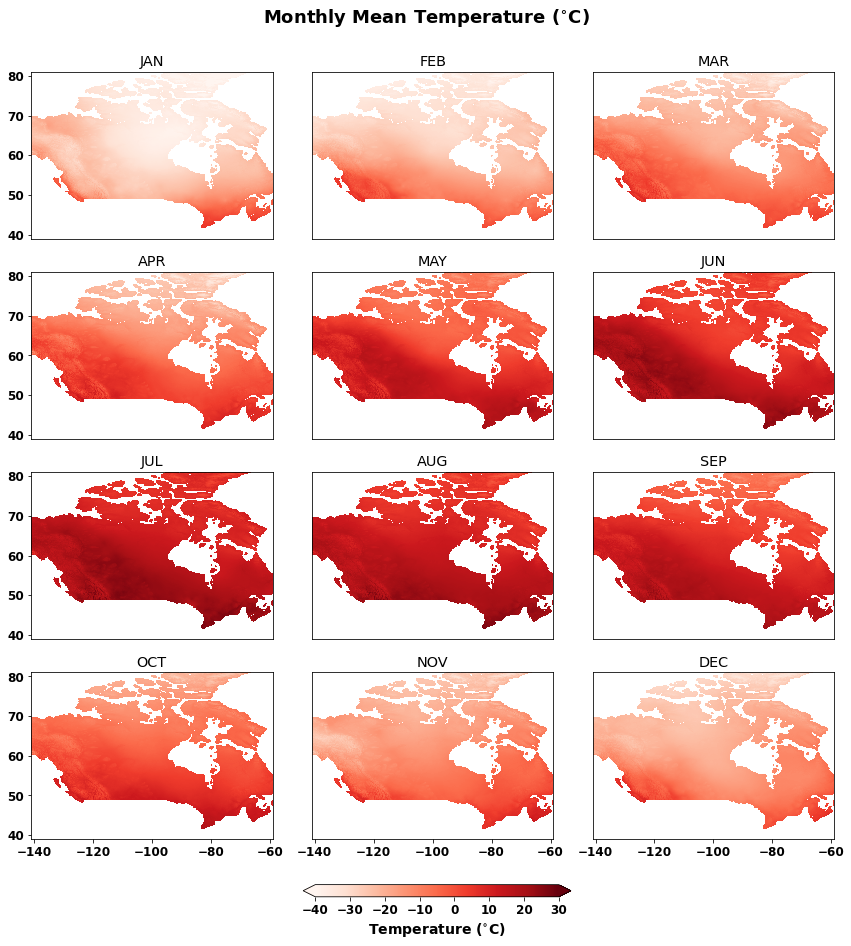
\includegraphics{output_11_0.png}
\caption{png}
\end{figure}

We can use the command \texttt{std(\textquotesingle{}time\textquotesingle{})} to calculate the standard deviation of the temperature over the time dimension.

\begin{Shaded}
\begin{Highlighting}[]
\NormalTok{t\_std }\OperatorTok{=}\NormalTok{ t\_daily.groupby(}\StringTok{\textquotesingle{}time.month\textquotesingle{}}\NormalTok{).std(}\StringTok{\textquotesingle{}time\textquotesingle{}}\NormalTok{).rename(\{}\StringTok{"tasmax"}\NormalTok{: }\StringTok{"t\_std"}\NormalTok{\})}
\end{Highlighting}
\end{Shaded}

Xarray also borrows some features from the pandas library to work on the time dimension. The code bellow calculates the mean temperature for each season.

\begin{Shaded}
\begin{Highlighting}[]
\NormalTok{t\_season }\OperatorTok{=}\NormalTok{ t\_daily.groupby(}\StringTok{\textquotesingle{}time.season\textquotesingle{}}\NormalTok{).mean(}\StringTok{\textquotesingle{}time\textquotesingle{}}\NormalTok{).rename(\{}\StringTok{"tasmax"}\NormalTok{: }\StringTok{"t\_mean"}\NormalTok{\})}
\NormalTok{t\_season}
\end{Highlighting}
\end{Shaded}

xarray.Dataset

Dimensions:

{lat}: 510

{lon}: 1068

{season}: 4

Coordinates: {(3)}

{lat}

(lat)

float64

41.04 41.12 41.21 \ldots{} 83.37 83.46

{long\_name :}

lat

{standard\_name :}

latitude

{NAME :}

lat

{units :}

degrees\_north

\_Netcdf4Dimid :

1

{CLASS :}

DIMENSION\_SCALE

{axis :}

Y

{lon}

(lon)

float64

-141.0 -140.9 \ldots{} -52.13 -52.04

{long\_name :}

lon

{standard\_name :}

longitude

{NAME :}

lon

{units :}

degrees\_east

\_Netcdf4Dimid :

0

{CLASS :}

DIMENSION\_SCALE

{axis :}

X

{season}

(season)

object

'DJF' 'JJA' 'MAM' 'SON'

Data variables: {(1)}

{t\_mean}

(season, lat, lon)

float32

nan nan nan nan \ldots{} nan nan nan nan

Attributes: {(0)}

This Dataset now has a new dimension \texttt{season} with 4 elements. We can now plot the seasonal mean temperature.

\begin{Shaded}
\begin{Highlighting}[]
\NormalTok{fig, axs }\OperatorTok{=}\NormalTok{ plt.subplots(}\DecValTok{2}\NormalTok{,}\DecValTok{2}\NormalTok{, figsize}\OperatorTok{=}\NormalTok{(}\DecValTok{12}\NormalTok{, }\DecValTok{14}\NormalTok{), facecolor}\OperatorTok{=}\StringTok{\textquotesingle{}w\textquotesingle{}}\NormalTok{, edgecolor}\OperatorTok{=}\StringTok{\textquotesingle{}k\textquotesingle{}}\NormalTok{)}
\NormalTok{fig.subplots\_adjust(hspace }\OperatorTok{=} \FloatTok{.0}\NormalTok{, wspace}\OperatorTok{=} \FloatTok{.2}\NormalTok{)}

\NormalTok{season }\OperatorTok{=}\NormalTok{ [}\StringTok{\textquotesingle{}DFJ\textquotesingle{}}\NormalTok{,}\StringTok{\textquotesingle{}JJA\textquotesingle{}}\NormalTok{,}\StringTok{\textquotesingle{}MAM\textquotesingle{}}\NormalTok{,}\StringTok{\textquotesingle{}SON\textquotesingle{}}\NormalTok{]}

\NormalTok{axs }\OperatorTok{=}\NormalTok{ axs.ravel()}

\ControlFlowTok{for}\NormalTok{ i }\KeywordTok{in} \BuiltInTok{range}\NormalTok{(}\BuiltInTok{len}\NormalTok{(season)):}
\NormalTok{    pc }\OperatorTok{=}\NormalTok{ axs[i].pcolormesh(t\_season.lon,t\_season.lat,t\_season[}\StringTok{\textquotesingle{}t\_mean\textquotesingle{}}\NormalTok{][i,:,:],cmap}\OperatorTok{=}\StringTok{"Reds"}\NormalTok{,vmin}\OperatorTok{={-}}\DecValTok{40}\NormalTok{,vmax}\OperatorTok{=}\DecValTok{40}\NormalTok{)}
\NormalTok{    axs[i].set\_title(season[i])}
\NormalTok{    axs[i].set\_ylim([}\DecValTok{39}\NormalTok{,}\DecValTok{81}\NormalTok{])}
\NormalTok{    axs[i].set\_xlim([}\OperatorTok{{-}}\DecValTok{141}\NormalTok{,}\OperatorTok{{-}}\DecValTok{59}\NormalTok{])}

    \ControlFlowTok{if}\NormalTok{ i }\KeywordTok{in}\NormalTok{ [}\DecValTok{0}\NormalTok{,}\DecValTok{2}\NormalTok{]:}
\NormalTok{        axs[i].set\_yticks([}\DecValTok{40}\NormalTok{,}\DecValTok{50}\NormalTok{,}\DecValTok{60}\NormalTok{,}\DecValTok{70}\NormalTok{,}\DecValTok{80}\NormalTok{])}
    \ControlFlowTok{else}\NormalTok{:}
\NormalTok{        axs[i].set\_yticks([])}

    \ControlFlowTok{if}\NormalTok{ i }\KeywordTok{in}\NormalTok{ [}\DecValTok{2}\NormalTok{,}\DecValTok{3}\NormalTok{]:}
\NormalTok{        axs[i].set\_xticks([}\OperatorTok{{-}}\DecValTok{140}\NormalTok{,}\OperatorTok{{-}}\DecValTok{120}\NormalTok{,}\OperatorTok{{-}}\DecValTok{100}\NormalTok{,}\OperatorTok{{-}}\DecValTok{80}\NormalTok{,}\OperatorTok{{-}}\DecValTok{60}\NormalTok{])}
    \ControlFlowTok{else}\NormalTok{:}
\NormalTok{        axs[i].set\_xticks([])                }

\NormalTok{fig.suptitle(}\StringTok{\textquotesingle{}Seasonal Mean Temperature ($\^{}\{\textbackslash{}circ\}$C)\textquotesingle{}}\NormalTok{,}
\NormalTok{             x}\OperatorTok{=}\FloatTok{0.5}\NormalTok{,y}\OperatorTok{=}\FloatTok{1.0}\NormalTok{,fontsize}\OperatorTok{=}\DecValTok{18}\NormalTok{,fontweight}\OperatorTok{=}\StringTok{"bold"}\NormalTok{)}

\NormalTok{cax,kw }\OperatorTok{=}\NormalTok{ mpl.colorbar.make\_axes(axs,location}\OperatorTok{=}\StringTok{\textquotesingle{}bottom\textquotesingle{}}\NormalTok{,pad}\OperatorTok{={-}}\FloatTok{0.48}\NormalTok{,shrink}\OperatorTok{=}\FloatTok{0.4}\NormalTok{)}
\NormalTok{out}\OperatorTok{=}\NormalTok{fig.colorbar(pc,cax}\OperatorTok{=}\NormalTok{cax,extend}\OperatorTok{=}\StringTok{\textquotesingle{}both\textquotesingle{}}\NormalTok{,}\OperatorTok{**}\NormalTok{kw)}

\NormalTok{out.set\_label(}\StringTok{"Temperature ($\^{}\{\textbackslash{}circ\}$C)"}\NormalTok{, fontweight}\OperatorTok{=}\StringTok{\textquotesingle{}bold\textquotesingle{}}\NormalTok{,fontsize}\OperatorTok{=}\DecValTok{14}\NormalTok{)}

\NormalTok{fig.tight\_layout()}
\NormalTok{plt.show()}
\end{Highlighting}
\end{Shaded}

\begin{figure}
\centering
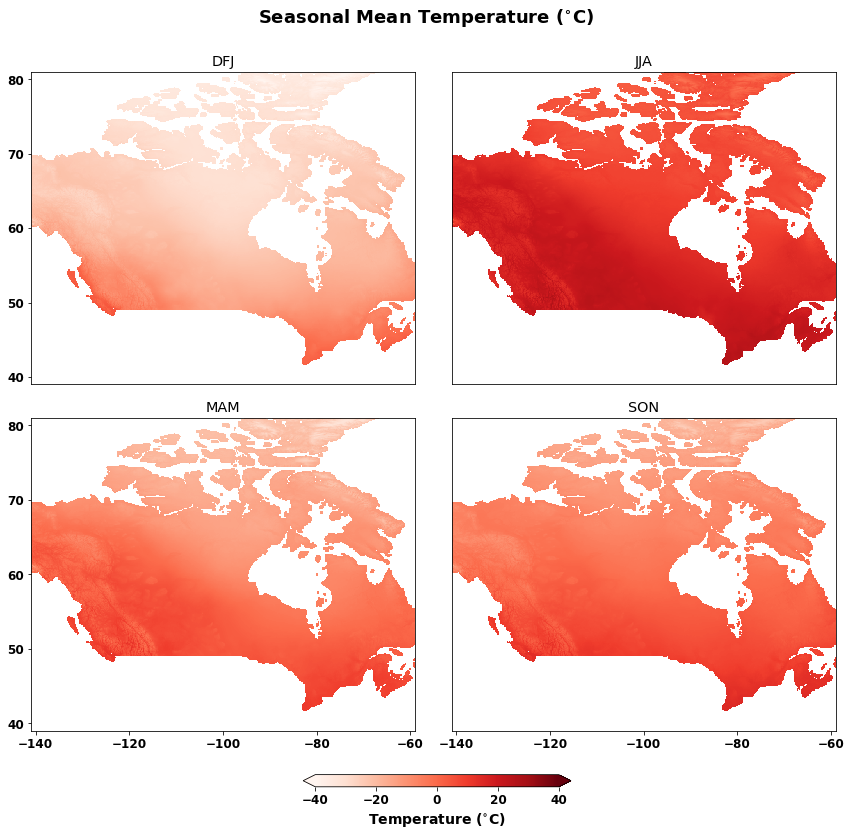
\includegraphics{output_17_0.png}
\caption{png}
\end{figure}

\hypertarget{multi-model-mean-in-xarray}{%
\section{\texorpdfstring{Multi-model mean in \emph{xarray}}{Multi-model mean in xarray}}\label{multi-model-mean-in-xarray}}

Now, let's say we have daily temperature data for 24 GCMs. How do we calculate the the mean over the time dimension for each model? We can do that by using a \texttt{for} loop as defined in the NumPy library.

For the sake of simplicity, the following code only enters the names of each one of the GCMs. Ultimately, you can use the command \texttt{xr.open\_dataset} to open the NetCDF files containing the daily data for each one of the models.

\begin{Shaded}
\begin{Highlighting}[]
\NormalTok{model\_name }\OperatorTok{=}\NormalTok{ [}\StringTok{"ACCESS1{-}0"}\NormalTok{,}\StringTok{"bcc{-}csm1{-}1"}\NormalTok{,}\StringTok{"bcc{-}csm1{-}1{-}m"}\NormalTok{,}\StringTok{"BNU{-}ESM"}\NormalTok{,}\StringTok{"CanESM2"}\NormalTok{,}\StringTok{"CCSM4"}\NormalTok{,}\StringTok{"CESM1{-}CAM5"}\NormalTok{,}
              \StringTok{"CNRM{-}CM5"}\NormalTok{,}\StringTok{"CSIRO{-}Mk3{-}6{-}0"}\NormalTok{,}\StringTok{"GFDL{-}CM3"}\NormalTok{,}\StringTok{"GFDL{-}ESM2G"}\NormalTok{,}\StringTok{"GFDL{-}ESM2M"}\NormalTok{,}\StringTok{"HadGEM2{-}AO"}\NormalTok{,}
              \StringTok{"HadGEM2{-}CC"}\NormalTok{,}\StringTok{"inmcm4"}\NormalTok{,}\StringTok{"IPSL{-}CM5A{-}LR"}\NormalTok{,}\StringTok{"IPSL{-}CM5A{-}MR"}\NormalTok{,}\StringTok{"MIROC5"}\NormalTok{,}\StringTok{"MIROC{-}ESM{-}CHEM"}\NormalTok{,}
              \StringTok{"MIROC{-}ESM"}\NormalTok{,}\StringTok{"MPI{-}ESM{-}LR"}\NormalTok{,}\StringTok{"MPI{-}ESM{-}MR"}\NormalTok{,}\StringTok{"MRI{-}CGCM3"}\NormalTok{,}\StringTok{"NorESM1{-}ME"}\NormalTok{,}\StringTok{"NorESM1{-}M"}\NormalTok{]}
\end{Highlighting}
\end{Shaded}

Before running the code, we need to import the pandas library. As discussed previously, the xarray library relies on several NumPy and pandas commands.

\begin{Shaded}
\begin{Highlighting}[]
\ImportTok{import}\NormalTok{ pandas }\ImportTok{as}\NormalTok{ pd}
\end{Highlighting}
\end{Shaded}

In the code below, we use the function \texttt{append()} to create a DataArray with average monthly temperature values for each GCM. In some way, we are creating a long array that contains the monthly average temperature for all 25 GCMs.

\begin{Shaded}
\begin{Highlighting}[]
\NormalTok{t\_model\_monthly}\OperatorTok{=}\NormalTok{[]}

\ControlFlowTok{for}\NormalTok{ file\_name }\KeywordTok{in}\NormalTok{ multimodel:}
\NormalTok{        t\_daily }\OperatorTok{=}\NormalTok{ xr.open\_mfdataset(file\_name)}
\NormalTok{        t\_mean }\OperatorTok{=}\NormalTok{ t\_daily.mean(}\StringTok{\textquotesingle{}time\textquotesingle{}}\NormalTok{)}
\NormalTok{        t\_model\_monthly.append(t\_mean)}
\end{Highlighting}
\end{Shaded}

However, the new variable \texttt{t\_mean\_monthly} is not very practical because xarray does not label the 25 GCMs under a new dimension \texttt{model} automatically. The Dataset created from the loop is a collection of 25 xarray objects. To create a new dimension, we can use the xarray function \texttt{xr.concat} to concatenate the xarray objects along a new or existing dimension. In this specific case, we want a new dimension.

\begin{Shaded}
\begin{Highlighting}[]
\NormalTok{t\_model\_monthly }\OperatorTok{=}\NormalTok{ xr.concat(t\_model\_monthly,pd.Index(}\BuiltInTok{range}\NormalTok{(}\DecValTok{25}\NormalTok{),name}\OperatorTok{=}\StringTok{\textquotesingle{}model\textquotesingle{}}\NormalTok{)).rename(\{}\StringTok{"tasmax"}\NormalTok{: }\StringTok{"t\_mean"}\NormalTok{\})}
\end{Highlighting}
\end{Shaded}

In this code, \texttt{pd.Index(range(25)} represents the new dimension added along axis=0.

The resulting Dataset is, thus, a new Dataset with a new dimension \texttt{model} wtih 25 elements on it.

\begin{Shaded}
\begin{Highlighting}[]
\NormalTok{t\_model\_monthly}
\end{Highlighting}
\end{Shaded}

xarray.Dataset

Dimensions:

{lat}: 510

{lon}: 1068

{model}: 25

Coordinates: {(3)}

{lat}

(lat)

float64

41.04 41.12 41.21 \ldots{} 83.37 83.46

{long\_name :}

latitude

{standard\_name :}

latitude

{NAME :}

lat

{units :}

degrees\_north

\_Netcdf4Dimid :

1

{CLASS :}

DIMENSION\_SCALE

{axis :}

Y

{lon}

(lon)

float64

-141.0 -140.9 \ldots{} -52.13 -52.04

{long\_name :}

longitude

{standard\_name :}

longitude

{NAME :}

lon

{units :}

degrees\_east

\_Netcdf4Dimid :

0

{CLASS :}

DIMENSION\_SCALE

{axis :}

X

{model}

(model)

int64

0 1 2 3 4 5 6 \ldots{} 19 20 21 22 23 24

Data variables: {(1)}

{t\_mean}

(model, lat, lon)

float32

dask.array\textless chunksize=(1, 510, 1068), meta=np.ndarray\textgreater{}

Array

Chunk

Bytes

51.94 MiB

2.08 MiB

Shape

(25, 510, 1068)

(1, 510, 1068)

Count

150 Tasks

25 Chunks

Type

float32

numpy.ndarray

1068
510
25

Attributes: {(0)}

Now, we plot the average temperature for each model.

\begin{Shaded}
\begin{Highlighting}[]
\NormalTok{fig, axs }\OperatorTok{=}\NormalTok{ plt.subplots(}\DecValTok{5}\NormalTok{,}\DecValTok{5}\NormalTok{, figsize}\OperatorTok{=}\NormalTok{(}\DecValTok{20}\NormalTok{, }\DecValTok{25}\NormalTok{), facecolor}\OperatorTok{=}\StringTok{\textquotesingle{}w\textquotesingle{}}\NormalTok{, edgecolor}\OperatorTok{=}\StringTok{\textquotesingle{}k\textquotesingle{}}\NormalTok{)}
\NormalTok{fig.subplots\_adjust(hspace }\OperatorTok{=} \FloatTok{.2}\NormalTok{, wspace}\OperatorTok{=} \FloatTok{.2}\NormalTok{)}

\NormalTok{axs }\OperatorTok{=}\NormalTok{ axs.ravel()}

\ControlFlowTok{for}\NormalTok{ i }\KeywordTok{in} \BuiltInTok{range}\NormalTok{(}\BuiltInTok{len}\NormalTok{(t\_model\_monthly[}\StringTok{\textquotesingle{}model\textquotesingle{}}\NormalTok{])):}

\NormalTok{    pc }\OperatorTok{=}\NormalTok{ axs[i].pcolormesh(t\_model\_monthly.lon,t\_model\_monthly.lat,t\_model\_monthly[}\StringTok{\textquotesingle{}t\_mean\textquotesingle{}}\NormalTok{][i,:,:],cmap}\OperatorTok{=}\StringTok{"Reds"}\NormalTok{)}
\NormalTok{    axs[i].set\_title(multimodel\_name[i])}
\NormalTok{    axs[i].set\_ylim([}\DecValTok{39}\NormalTok{,}\DecValTok{81}\NormalTok{])}
\NormalTok{    axs[i].set\_xlim([}\OperatorTok{{-}}\DecValTok{141}\NormalTok{,}\OperatorTok{{-}}\DecValTok{59}\NormalTok{])}
\NormalTok{    axs[i].set\_yticks([}\DecValTok{40}\NormalTok{,}\DecValTok{50}\NormalTok{,}\DecValTok{60}\NormalTok{,}\DecValTok{70}\NormalTok{,}\DecValTok{80}\NormalTok{])}
\NormalTok{    axs[i].set\_xticks([}\OperatorTok{{-}}\DecValTok{140}\NormalTok{,}\OperatorTok{{-}}\DecValTok{120}\NormalTok{,}\OperatorTok{{-}}\DecValTok{100}\NormalTok{,}\OperatorTok{{-}}\DecValTok{80}\NormalTok{,}\OperatorTok{{-}}\DecValTok{60}\NormalTok{])}
\NormalTok{    cax,kw }\OperatorTok{=}\NormalTok{ mpl.colorbar.make\_axes(axs[i],location}\OperatorTok{=}\StringTok{\textquotesingle{}bottom\textquotesingle{}}\NormalTok{)}\CommentTok{\#,pad=0.05,shrink=0.7)}
\NormalTok{    out}\OperatorTok{=}\NormalTok{fig.colorbar(pc,cax}\OperatorTok{=}\NormalTok{cax,extend}\OperatorTok{=}\StringTok{\textquotesingle{}both\textquotesingle{}}\NormalTok{,}\OperatorTok{**}\NormalTok{kw)    }\CommentTok{\#axs[i].axis("tight")}

\NormalTok{fig.suptitle(}\StringTok{\textquotesingle{}Mean Temperature ($\^{}\{\textbackslash{}circ\}$C) for each GCM\textquotesingle{}}\NormalTok{,}
\NormalTok{             x}\OperatorTok{=}\FloatTok{0.5}\NormalTok{,y}\OperatorTok{=}\FloatTok{0.91}\NormalTok{,fontsize}\OperatorTok{=}\DecValTok{18}\NormalTok{,fontweight}\OperatorTok{=}\StringTok{"bold"}\NormalTok{)}

\CommentTok{\#fig.tight\_layout()}
\NormalTok{plt.show()}
\end{Highlighting}
\end{Shaded}

\begin{figure}
\centering
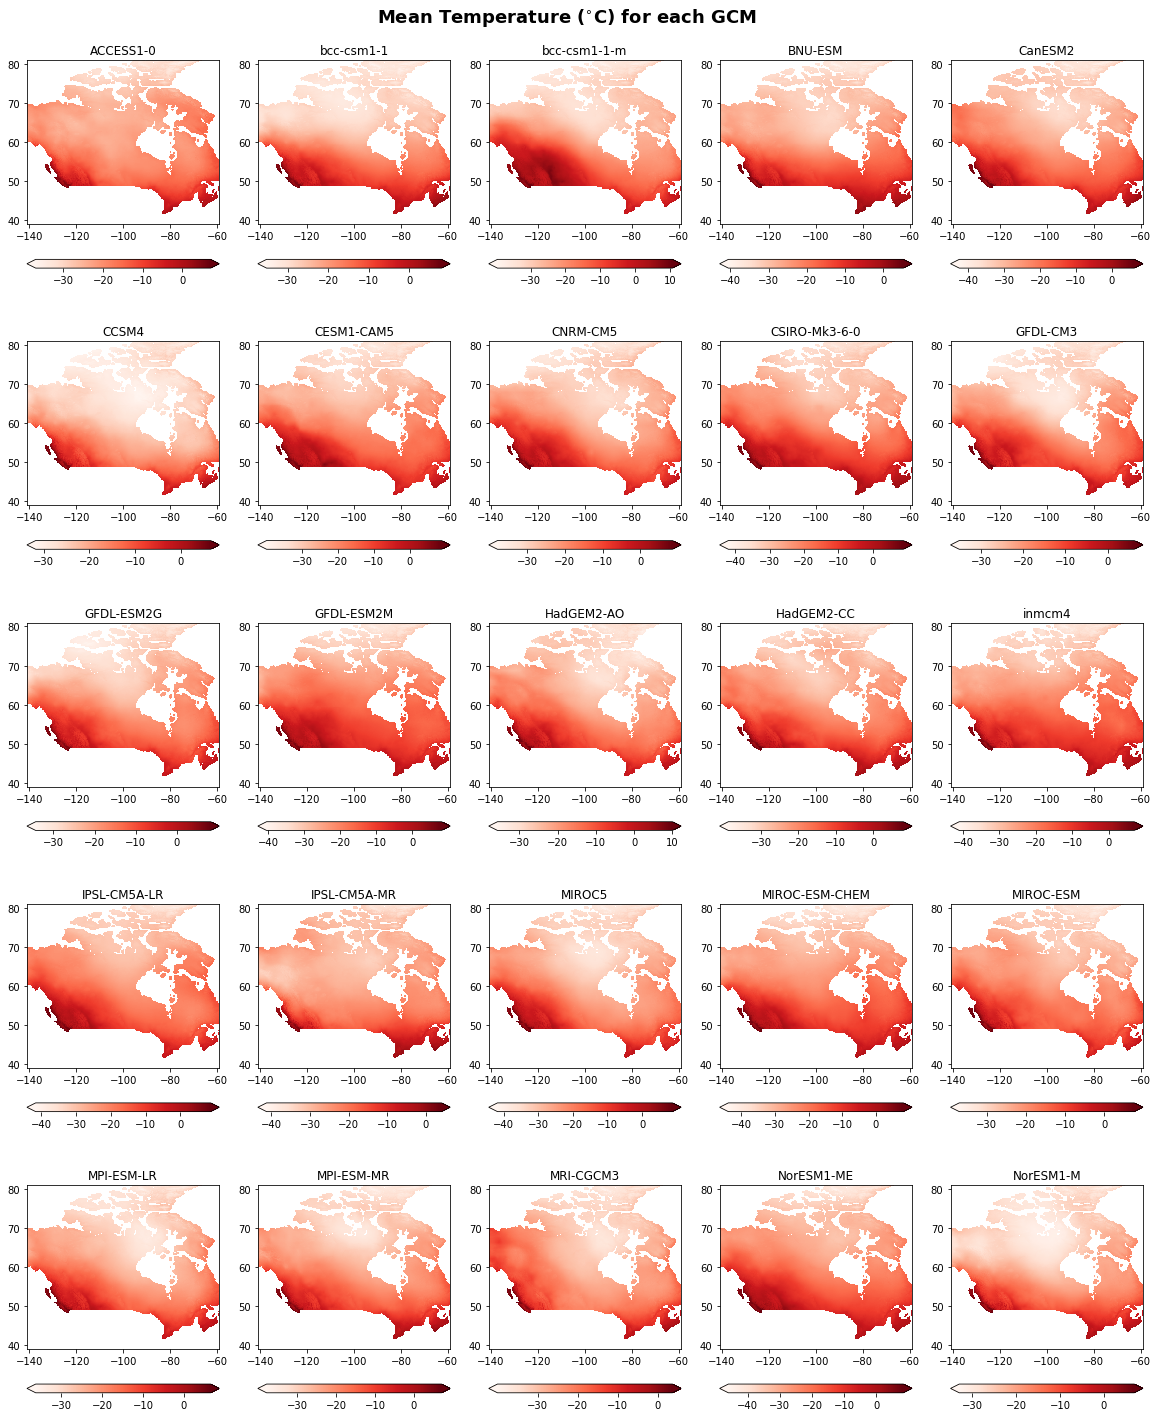
\includegraphics{output_15_0.png}
\caption{Figure 1 - Mean temperature calculated for each GCM}
\end{figure}

The beauty of creating a new dimension \texttt{model} to store the values for each model is that we can easily calculate the multi-model ensemble mean temperature by simply executing the operation \texttt{mean()} over the model dimension.

\begin{Shaded}
\begin{Highlighting}[]
\NormalTok{t\_ensemble }\OperatorTok{=}\NormalTok{ t\_model\_monthly.mean(}\StringTok{\textquotesingle{}model\textquotesingle{}}\NormalTok{)}
\end{Highlighting}
\end{Shaded}

xarray.Dataset

Dimensions:

{lat}: 510

{lon}: 1068

Coordinates: {(2)}

{lat}

(lat)

float64

41.04 41.12 41.21 \ldots{} 83.37 83.46

{long\_name :}

latitude

{standard\_name :}

latitude

{NAME :}

lat

{units :}

degrees\_north

\_Netcdf4Dimid :

1

{CLASS :}

DIMENSION\_SCALE

{axis :}

Y

{lon}

(lon)

float64

-141.0 -140.9 \ldots{} -52.13 -52.04

{long\_name :}

longitude

{standard\_name :}

longitude

{NAME :}

lon

{units :}

degrees\_east

\_Netcdf4Dimid :

0

{CLASS :}

DIMENSION\_SCALE

{axis :}

X

Data variables: {(1)}

{t\_mean}

(lat, lon)

float32

nan nan nan nan \ldots{} nan nan nan nan

Attributes: {(0)}

Finally, we can plot the multi-model ensemble mean.

\begin{Shaded}
\begin{Highlighting}[]
\NormalTok{fig }\OperatorTok{=}\NormalTok{ plt.figure(figsize}\OperatorTok{=}\NormalTok{(}\DecValTok{16}\NormalTok{,}\DecValTok{12}\NormalTok{))}
\NormalTok{ax }\OperatorTok{=}\NormalTok{ plt.axes(projection}\OperatorTok{=}\NormalTok{ccrs.PlateCarree())}
\CommentTok{\#ax.set\_global()}
\NormalTok{ax.coastlines()}
\NormalTok{ax.gridlines(linewidth}\OperatorTok{=}\DecValTok{1}\NormalTok{)}
\NormalTok{gl }\OperatorTok{=}\NormalTok{ ax.gridlines(crs}\OperatorTok{=}\NormalTok{ccrs.PlateCarree(), draw\_labels}\OperatorTok{=}\VariableTok{True}\NormalTok{,}
\NormalTok{                 linewidth}\OperatorTok{=}\DecValTok{1}\NormalTok{, color}\OperatorTok{=}\StringTok{\textquotesingle{}darkgrey\textquotesingle{}}\NormalTok{)}
\NormalTok{gl.xlabels\_top }\OperatorTok{=} \VariableTok{False}
\NormalTok{gl.ylabels\_left }\OperatorTok{=} \VariableTok{False}
\NormalTok{gl.xformatter }\OperatorTok{=}\NormalTok{ LONGITUDE\_FORMATTER}
\NormalTok{gl.yformatter }\OperatorTok{=}\NormalTok{ LATITUDE\_FORMATTER}
\NormalTok{gl.xlabel\_style }\OperatorTok{=}\NormalTok{ \{}\StringTok{\textquotesingle{}size\textquotesingle{}}\NormalTok{: }\DecValTok{15}\NormalTok{, }\StringTok{\textquotesingle{}color\textquotesingle{}}\NormalTok{: }\StringTok{\textquotesingle{}gray\textquotesingle{}}\NormalTok{\}}
\NormalTok{gl.xlabel\_style }\OperatorTok{=}\NormalTok{ \{}\StringTok{\textquotesingle{}color\textquotesingle{}}\NormalTok{: }\StringTok{\textquotesingle{}black\textquotesingle{}}\NormalTok{, }\StringTok{\textquotesingle{}weight\textquotesingle{}}\NormalTok{: }\StringTok{\textquotesingle{}bold\textquotesingle{}}\NormalTok{\}}

\CommentTok{\# uncomment and complete the line below (see the NAO notebook for a reminder)}
\NormalTok{pc }\OperatorTok{=}\NormalTok{ ax.pcolormesh(t\_ensemble.lon,t\_ensemble.lat,t\_ensemble[}\StringTok{\textquotesingle{}t\_mean\textquotesingle{}}\NormalTok{],cmap}\OperatorTok{=}\StringTok{"Reds"}\NormalTok{)}
\NormalTok{cax,kw }\OperatorTok{=}\NormalTok{ mpl.colorbar.make\_axes(ax,location}\OperatorTok{=}\StringTok{\textquotesingle{}bottom\textquotesingle{}}\NormalTok{,pad}\OperatorTok{=}\FloatTok{0.05}\NormalTok{,shrink}\OperatorTok{=}\FloatTok{0.7}\NormalTok{)}
\NormalTok{out}\OperatorTok{=}\NormalTok{fig.colorbar(pc,cax}\OperatorTok{=}\NormalTok{cax,extend}\OperatorTok{=}\StringTok{\textquotesingle{}both\textquotesingle{}}\NormalTok{,}\OperatorTok{**}\NormalTok{kw)}
\NormalTok{out.set\_label(}\StringTok{\textquotesingle{}Temperature ($\^{}\{\textbackslash{}circ\}$C)\textquotesingle{}}\NormalTok{,size}\OperatorTok{=}\DecValTok{14}\NormalTok{)}
\NormalTok{ax.set\_title(}\StringTok{\textquotesingle{}Multi{-}Model Ensemble Mean Temperature ($\^{}\{\textbackslash{}circ\}$C)\textquotesingle{}}\NormalTok{,pad }\OperatorTok{=} \DecValTok{15}\NormalTok{,fontweight}\OperatorTok{=}\StringTok{\textquotesingle{}bold\textquotesingle{}}\NormalTok{,size}\OperatorTok{=}\DecValTok{16}\NormalTok{)}
\end{Highlighting}
\end{Shaded}

\begin{figure}
\centering
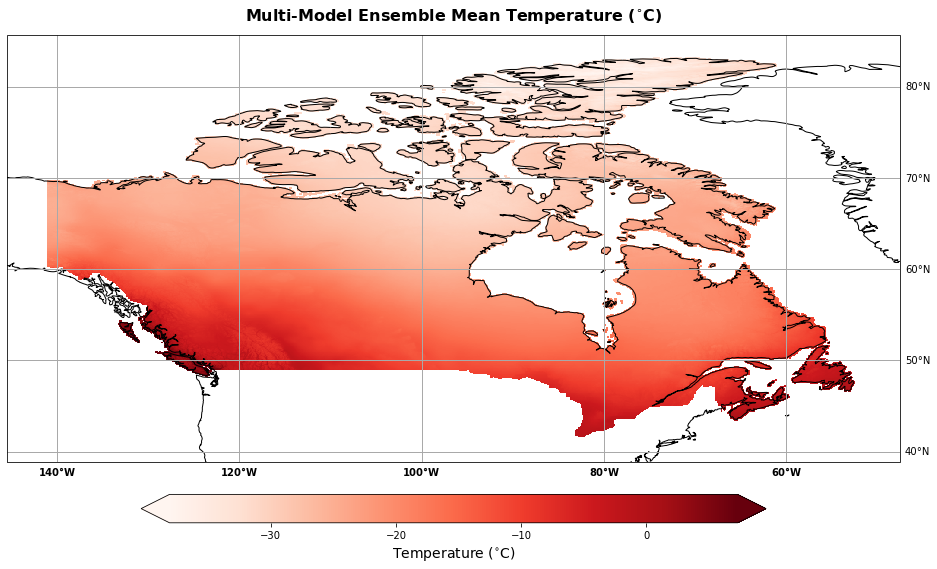
\includegraphics{output_19_1.png}
\caption{Figure 2 - Multi-model mean temperature}
\end{figure}

\hypertarget{calculating-autocorrelation-lag-1}{%
\section{Calculating autocorrelation lag-1}\label{calculating-autocorrelation-lag-1}}

In the last two section, we saw how to use the well-defined NumPy operations \texttt{mean()} and \texttt{std()} in a Dataset over the dimension \texttt{time}. Now, how would we create new a function that is not defined in the NumPy library? Let's try first with the lag-1 autocorrelation.

First, let's define create a new function \texttt{lag1\_numpy} by using the NumPy syntax.

\begin{Shaded}
\begin{Highlighting}[]
\KeywordTok{def}\NormalTok{ lag1\_numpy(array):}
\NormalTok{    ecorr }\OperatorTok{=}\NormalTok{ np.correlate((array}\OperatorTok{{-}}\NormalTok{np.mean(array))}\OperatorTok{/}\NormalTok{np.std(array),(array}\OperatorTok{{-}}\NormalTok{np.mean(array))}
                         \OperatorTok{/}\NormalTok{np.std(array),}\StringTok{\textquotesingle{}same\textquotesingle{}}\NormalTok{)}\OperatorTok{/}\BuiltInTok{len}\NormalTok{(array)}
\NormalTok{    lag1\_numpy }\OperatorTok{=}\NormalTok{ ecorr[}\BuiltInTok{int}\NormalTok{(}\BuiltInTok{len}\NormalTok{(ecorr)}\OperatorTok{/}\DecValTok{2}\NormalTok{)}\OperatorTok{+}\DecValTok{1}\NormalTok{]}
    \ControlFlowTok{return}\NormalTok{ lag1\_numpy}
\end{Highlighting}
\end{Shaded}

This function is taking an \texttt{array} and applying the NumPy operation \texttt{ecorr}.

Now, we define an xarray function by using the command \texttt{xr.apply\_ufunc}. Fundamentally, this command allows for executing a NumPy function over a Dataset. It is a powerful tool because it fills a gap whenever the xarray library lacks a built-in function. However, it comes with several trade-offs that will be discussed over this section and the next.

\begin{Shaded}
\begin{Highlighting}[]
\KeywordTok{def}\NormalTok{ lag1\_xarrray(array,dim}\OperatorTok{=}\StringTok{"time"}\NormalTok{):}
\NormalTok{    lag1\_xarrray }\OperatorTok{=}\NormalTok{ xr.apply\_ufunc(lag1\_numpy,array,}
\NormalTok{                     input\_core\_dims}\OperatorTok{=}\NormalTok{[[dim]], }
\NormalTok{                     vectorize}\OperatorTok{=}\VariableTok{True}\NormalTok{)}
    \ControlFlowTok{return}\NormalTok{ lag1\_xarrray}
\end{Highlighting}
\end{Shaded}

In the code above, we defined a function \texttt{lag1\_xarrray} that executes \texttt{lag1\_numpy} over the time dimension of a Dataset.

Now, let's consider calculate the lag-1 autocorrelation of daily temperature of 25 GCMs. As described

\begin{Shaded}
\begin{Highlighting}[]
\NormalTok{lag1\_model}\OperatorTok{=}\NormalTok{[]}

\ControlFlowTok{for}\NormalTok{ file\_name }\KeywordTok{in}\NormalTok{ multimodel:}
\NormalTok{        t\_daily }\OperatorTok{=}\NormalTok{ xr.open\_dataset(file\_name)}
\NormalTok{        lag1 }\OperatorTok{=}\NormalTok{ lag1\_xarrray(t\_daily[}\StringTok{\textquotesingle{}tasmax\textquotesingle{}}\NormalTok{])}
\NormalTok{        lag1\_model.append(lag1)}
\end{Highlighting}
\end{Shaded}

As discussed in the previous section, xarray does not automatically a new dimension \texttt{model} when we simply loop over 25 NetCDF files. At this moment, our Dataset \texttt{lag1\_model} is a collection of 25 DataArrays that is not very useful for other purposes. In this case, we cannot simply create a new dimension with \texttt{xr.concat} because we lost some information about our variable along the way when using the function \texttt{lag1\_xarrray}.

In this case, we can use the function \texttt{xr.Dataset} to manually create a new variable \texttt{lag1} over a new dimension \texttt{model}.

\begin{Shaded}
\begin{Highlighting}[]
\NormalTok{lag1\_model }\OperatorTok{=}\NormalTok{ xr.Dataset(}
\NormalTok{    data\_vars}\OperatorTok{=}\NormalTok{\{}
        \StringTok{"lag1"}\NormalTok{: ((}\StringTok{"model"}\NormalTok{,}\StringTok{"lat"}\NormalTok{, }\StringTok{"lon"}\NormalTok{), lag1\_model.data),}
\NormalTok{    \},}
\NormalTok{    coords}\OperatorTok{=}\NormalTok{\{}
        \StringTok{"model"}\NormalTok{: }\BuiltInTok{range}\NormalTok{(}\DecValTok{25}\NormalTok{),}
        \StringTok{"lat"}\NormalTok{: lag1\_model.lat,}
        \StringTok{"lon"}\NormalTok{: lag1\_model.lon,}
\NormalTok{    \},}
\NormalTok{    attrs }\OperatorTok{=} \BuiltInTok{dict}\NormalTok{(}
\NormalTok{        variable}\OperatorTok{=}\StringTok{"Autocorrelation lag{-}1"}\NormalTok{,}
\NormalTok{        description}\OperatorTok{=}\StringTok{"CMIP5 Models Data"}\NormalTok{,}
\NormalTok{        units}\OperatorTok{=}\StringTok{"{-}"}\NormalTok{))}
\end{Highlighting}
\end{Shaded}

Now we have a Dataset with with a new dimension \texttt{model} and variable \texttt{lag1}.

\begin{Shaded}
\begin{Highlighting}[]
\NormalTok{lag1\_model}
\end{Highlighting}
\end{Shaded}

xarray.Dataset

Dimensions:

{model}: 25

{lat}: 510

{lon}: 1068

Coordinates: {(3)}

{model}

(model)

int64

0 1 2 3 4 5 6 \ldots{} 19 20 21 22 23 24

{lat}

(lat)

float64

41.04 41.12 41.21 \ldots{} 83.37 83.46

{long\_name :}

latitude

{standard\_name :}

latitude

{NAME :}

lat

{units :}

degrees\_north

\_Netcdf4Dimid :

1

{CLASS :}

DIMENSION\_SCALE

{axis :}

Y

{lon}

(lon)

float64

-141.0 -140.9 \ldots{} -52.13 -52.04

{long\_name :}

longitude

{standard\_name :}

longitude

{NAME :}

lon

{units :}

degrees\_east

\_Netcdf4Dimid :

0

{CLASS :}

DIMENSION\_SCALE

{axis :}

X

Data variables: {(1)}

{lag1}

(model, lat, lon)

float32

nan nan nan nan \ldots{} nan nan nan nan

Attributes: {(3)}

{variable :}

Daily Near-Surface Maximum Air Temperature

{description :}

CMIP5 Models Data

{units :}

degC

As you probably noticed, it took a long time to run the loop with the function \texttt{lag1\_xarrray}. This is a problem that can be potentially mitigated by using some features of the Dask library that are integrated into the xarray library. For now, we are just going to plot the multi-model ensemble lag-1 autocorrelation and discuss these features in the next section.

\begin{Shaded}
\begin{Highlighting}[]
\NormalTok{lag1\_multimodel }\OperatorTok{=}\NormalTok{ lag1\_model.mean(}\StringTok{\textquotesingle{}model\textquotesingle{}}\NormalTok{)}
\end{Highlighting}
\end{Shaded}

xarray.Dataset

Dimensions:

{lat}: 510

{lon}: 1068

Coordinates: {(2)}

{lat}

(lat)

float64

41.04 41.12 41.21 \ldots{} 83.37 83.46

{long\_name :}

latitude

{standard\_name :}

latitude

{NAME :}

lat

{units :}

degrees\_north

\_Netcdf4Dimid :

1

{CLASS :}

DIMENSION\_SCALE

{axis :}

Y

{lon}

(lon)

float64

-141.0 -140.9 \ldots{} -52.13 -52.04

{long\_name :}

longitude

{standard\_name :}

longitude

{NAME :}

lon

{units :}

degrees\_east

\_Netcdf4Dimid :

0

{CLASS :}

DIMENSION\_SCALE

{axis :}

X

Data variables: {(1)}

{lag1}

(lat, lon)

float32

nan nan nan nan \ldots{} nan nan nan nan

Attributes: {(0)}

Finally, we can plot the multi-model ensemble lag-1 autocorrelation.

\begin{Shaded}
\begin{Highlighting}[]
\NormalTok{fig }\OperatorTok{=}\NormalTok{ plt.figure(figsize}\OperatorTok{=}\NormalTok{(}\DecValTok{16}\NormalTok{,}\DecValTok{12}\NormalTok{))}
\NormalTok{ax }\OperatorTok{=}\NormalTok{ plt.axes(projection}\OperatorTok{=}\NormalTok{ccrs.PlateCarree())}
\NormalTok{ax.coastlines()}
\NormalTok{ax.gridlines(linewidth}\OperatorTok{=}\DecValTok{1}\NormalTok{)}
\NormalTok{gl }\OperatorTok{=}\NormalTok{ ax.gridlines(crs}\OperatorTok{=}\NormalTok{ccrs.PlateCarree(), draw\_labels}\OperatorTok{=}\VariableTok{True}\NormalTok{,}
\NormalTok{                 linewidth}\OperatorTok{=}\DecValTok{1}\NormalTok{, color}\OperatorTok{=}\StringTok{\textquotesingle{}darkgrey\textquotesingle{}}\NormalTok{)}
\NormalTok{gl.xlabels\_top }\OperatorTok{=} \VariableTok{False}
\NormalTok{gl.ylabels\_left }\OperatorTok{=} \VariableTok{False}
\NormalTok{gl.xformatter }\OperatorTok{=}\NormalTok{ LONGITUDE\_FORMATTER}
\NormalTok{gl.yformatter }\OperatorTok{=}\NormalTok{ LATITUDE\_FORMATTER}
\NormalTok{gl.xlabel\_style }\OperatorTok{=}\NormalTok{ \{}\StringTok{\textquotesingle{}size\textquotesingle{}}\NormalTok{: }\DecValTok{15}\NormalTok{, }\StringTok{\textquotesingle{}color\textquotesingle{}}\NormalTok{: }\StringTok{\textquotesingle{}gray\textquotesingle{}}\NormalTok{\}}
\NormalTok{gl.xlabel\_style }\OperatorTok{=}\NormalTok{ \{}\StringTok{\textquotesingle{}color\textquotesingle{}}\NormalTok{: }\StringTok{\textquotesingle{}black\textquotesingle{}}\NormalTok{, }\StringTok{\textquotesingle{}weight\textquotesingle{}}\NormalTok{: }\StringTok{\textquotesingle{}bold\textquotesingle{}}\NormalTok{\}}

\NormalTok{pc }\OperatorTok{=}\NormalTok{ ax.pcolormesh(lag1\_multimodel.lon,lag1\_multimodel.lat,lag1\_multimodel[}\StringTok{\textquotesingle{}lag1\textquotesingle{}}\NormalTok{],cmap}\OperatorTok{=}\StringTok{"Reds"}\NormalTok{)}
\NormalTok{cax,kw }\OperatorTok{=}\NormalTok{ mpl.colorbar.make\_axes(ax,location}\OperatorTok{=}\StringTok{\textquotesingle{}bottom\textquotesingle{}}\NormalTok{,pad}\OperatorTok{=}\FloatTok{0.05}\NormalTok{,shrink}\OperatorTok{=}\FloatTok{0.7}\NormalTok{)}
\NormalTok{out}\OperatorTok{=}\NormalTok{fig.colorbar(pc,cax}\OperatorTok{=}\NormalTok{cax,extend}\OperatorTok{=}\StringTok{\textquotesingle{}both\textquotesingle{}}\NormalTok{,}\OperatorTok{**}\NormalTok{kw)}
\NormalTok{out.set\_label(}\StringTok{\textquotesingle{}Lag 1\textquotesingle{}}\NormalTok{,size}\OperatorTok{=}\DecValTok{14}\NormalTok{)}
\NormalTok{ax.set\_title(}\StringTok{\textquotesingle{}Multi{-}Model Ensemble Lag{-}1 Autocorrelation\textquotesingle{}}\NormalTok{, }
\NormalTok{             pad }\OperatorTok{=} \DecValTok{15}\NormalTok{,fontweight}\OperatorTok{=}\StringTok{\textquotesingle{}bold\textquotesingle{}}\NormalTok{,size}\OperatorTok{=}\DecValTok{16}\NormalTok{)}
\end{Highlighting}
\end{Shaded}

\begin{figure}
\centering
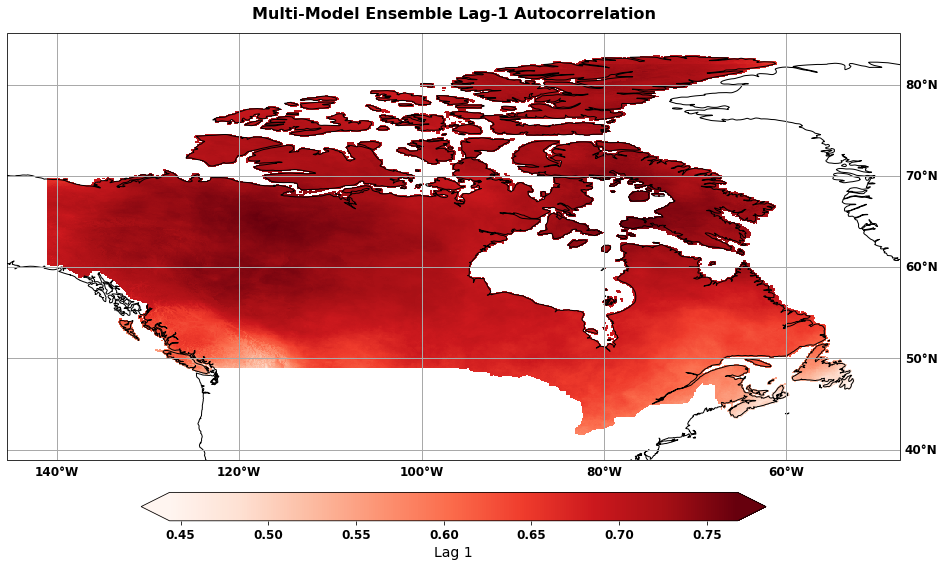
\includegraphics{output_16_1.png}
\caption{png}
\end{figure}

\hypertarget{dask-arrays-and-parallel-calculations}{%
\section{\texorpdfstring{\emph{Dask} arrays and parallel calculations}{Dask arrays and parallel calculations}}\label{dask-arrays-and-parallel-calculations}}

Now, let's create a function that calculates the e-folding time. First, we define this function with NumPy syntax.

\begin{Shaded}
\begin{Highlighting}[]
\KeywordTok{def}\NormalTok{ efold\_numpy(array):}
\NormalTok{    ecorr }\OperatorTok{=}\NormalTok{ np.correlate((array}\OperatorTok{{-}}\NormalTok{np.mean(array))}\OperatorTok{/}\NormalTok{np.std(array),(array}\OperatorTok{{-}}\NormalTok{np.mean(array))}
                         \OperatorTok{/}\NormalTok{np.std(array),}\StringTok{\textquotesingle{}same\textquotesingle{}}\NormalTok{)}\OperatorTok{/}\BuiltInTok{len}\NormalTok{(array)}
\NormalTok{    lag1 }\OperatorTok{=}\NormalTok{ ecorr[}\BuiltInTok{int}\NormalTok{(}\BuiltInTok{len}\NormalTok{(ecorr)}\OperatorTok{/}\DecValTok{2}\NormalTok{)}\OperatorTok{+}\DecValTok{1}\NormalTok{]}
\NormalTok{    efold\_numpy }\OperatorTok{=} \OperatorTok{{-}}\DecValTok{1}\OperatorTok{/}\NormalTok{np.log(lag1)}
    \ControlFlowTok{return}\NormalTok{ efold\_numpy}
\end{Highlighting}
\end{Shaded}

Now, we are going to use the function \texttt{xr.apply\_ufunc} and there are two important features to consider when using Dask. Firstly, we have to execute parallel calculation by including \texttt{dask="parallelized"} and \texttt{allow\_rechunk\ =\ True} in the function.

\begin{Shaded}
\begin{Highlighting}[]
\KeywordTok{def}\NormalTok{ efold\_xarray(array):}
\NormalTok{    efold\_xarray }\OperatorTok{=}\NormalTok{ xr.apply\_ufunc(}
\NormalTok{            efold\_numpy, }
\NormalTok{            t\_daily.groupby(}\StringTok{\textquotesingle{}time.month\textquotesingle{}}\NormalTok{), }
\NormalTok{            input\_core\_dims}\OperatorTok{=}\NormalTok{[[}\StringTok{"time"}\NormalTok{]],  }
\NormalTok{            exclude\_dims}\OperatorTok{=}\BuiltInTok{set}\NormalTok{((}\StringTok{"time"}\NormalTok{,)),}
\NormalTok{            vectorize}\OperatorTok{=}\VariableTok{True}\NormalTok{,  }
\NormalTok{            dask}\OperatorTok{=}\StringTok{"parallelized"}\NormalTok{,}
\NormalTok{            dask\_gufunc\_kwargs }\OperatorTok{=} \BuiltInTok{dict}\NormalTok{(allow\_rechunk }\OperatorTok{=} \VariableTok{True}\NormalTok{),}
\NormalTok{            output\_dtypes}\OperatorTok{=}\NormalTok{[array[}\StringTok{\textquotesingle{}tasmax\textquotesingle{}}\NormalTok{].dtype]).rename(\{}\StringTok{"tasmax"}\NormalTok{: }\StringTok{"efold"}\NormalTok{\})}
    \ControlFlowTok{return}\NormalTok{ efold\_xarray}
\end{Highlighting}
\end{Shaded}

Secondly, we have to define the size of our chunks when opening the NetCDF files. By specifying the chunk shape, xarray will automatically create Dask arrays for each data variable in the Dataset.

\begin{Shaded}
\begin{Highlighting}[]
\NormalTok{efold\_model }\OperatorTok{=}\NormalTok{ []}

\ControlFlowTok{for}\NormalTok{ file\_name }\KeywordTok{in}\NormalTok{ multimodel:}
\NormalTok{        t\_daily }\OperatorTok{=}\NormalTok{ xr.open\_dataset(file\_name,chunks}\OperatorTok{=}\NormalTok{\{}\StringTok{"lat"}\NormalTok{: }\DecValTok{150}\NormalTok{, }\StringTok{"lon"}\NormalTok{: }\DecValTok{200}\NormalTok{\})}
\NormalTok{        efold }\OperatorTok{=}\NormalTok{ efold\_xarray(t\_daily)}
\NormalTok{        efold\_model.append(efold)}

\NormalTok{efold\_model }\OperatorTok{=}\NormalTok{ xr.concat(efold\_model,pd.Index(}\BuiltInTok{range}\NormalTok{(}\DecValTok{25}\NormalTok{),name}\OperatorTok{=}\StringTok{\textquotesingle{}model\textquotesingle{}}\NormalTok{))}
\end{Highlighting}
\end{Shaded}

xarray.Dataset

Dimensions:

{month}: 2

{model}: 25

{lat}: 510

{lon}: 1068

Coordinates: {(4)}

{month}

(month)

int64

1 2

{lat}

(lat)

float64

41.04 41.12 41.21 \ldots{} 83.37 83.46

{lon}

(lon)

float64

-141.0 -140.9 \ldots{} -52.13 -52.04

{model}

(model)

int64

0 1 2 3 4 5 6 \ldots{} 19 20 21 22 23 24

Data variables: {(1)}

{efold}

(model, month, lat, lon)

float32

dask.array\textless chunksize=(1, 1, 150, 200), meta=np.ndarray\textgreater{}

Array

Chunk

Bytes

103.89 MiB

117.19 kiB

Shape

(25, 2, 510, 1068)

(1, 1, 150, 200)

Count

9291 Tasks

1200 Chunks

Type

float32

numpy.ndarray

25
1

1068
510
2

Attributes: {(0)}

As you probably noticed, it took a few seconds (or less) to execute the \texttt{efold\_xarray} and create a new Dataset with the variable \texttt{efold} and a new dimension \texttt{model}. From a user standpoint, the key concept of a \texttt{dask.array} is the notion of chunk. A chunk is the user-defined shape of the subdataset on which the unitary tasks will be applied.

Building upon dask has several advantages. For instance, the only modification of your code that is needed is your defining the chunks on which the computation should be performed. The Dask library also allows to easily leverage the resources of shared memory architectures (multi-core laptop or work-station) but also the resources of distributed memory architectures (clusters of cpu).

Yet, parallelization comes at a cost. Loading the data with dask.arrays is only done at the execution time if needed. This means that we have access to this Dataset without having to worry about time time it will take to load the data. The chunks also have implications on the performance of the code. If the chunks are too small, queueing up operations will be extremely slow, because Dask will translate each operation into a huge number of operations mapped across chunks. If the chunks are too big, some of the computation power may be wasted, because Dask only computes results one chunk at a time.

\hypertarget{key-takeaways}{%
\chapter{Key takeaways}\label{key-takeaways}}

  \bibliography{book.bib,packages.bib}

\end{document}
